\chapter{Dz Covid Traker}

\section{OverView}
COVID-19 may not be the first pandemic the world has faced, but the virus' challenge comes amidst widespread skepticism of longstanding public health institutions.\\

Government-led responses to outbreaks have varied from country to country, and incongruent messaging between political leaders, health agencies and other sources of information have fueled varying levels of concern and distrust among individuals seeking to protect themselves from the disease.\\

Perhaps unsurprisingly, these past several months have also seen an extensive range of novel technologies released to help educate worried consumers or connect isolated patients to testing or care.\\

Among the best known of these tools are contact tracing and symptom-reporting apps, some of which are increasingly being deployed by local and national public health agencies
\newpage
\section{The association entity model:}


\begin{figure}[!htb]
        \center{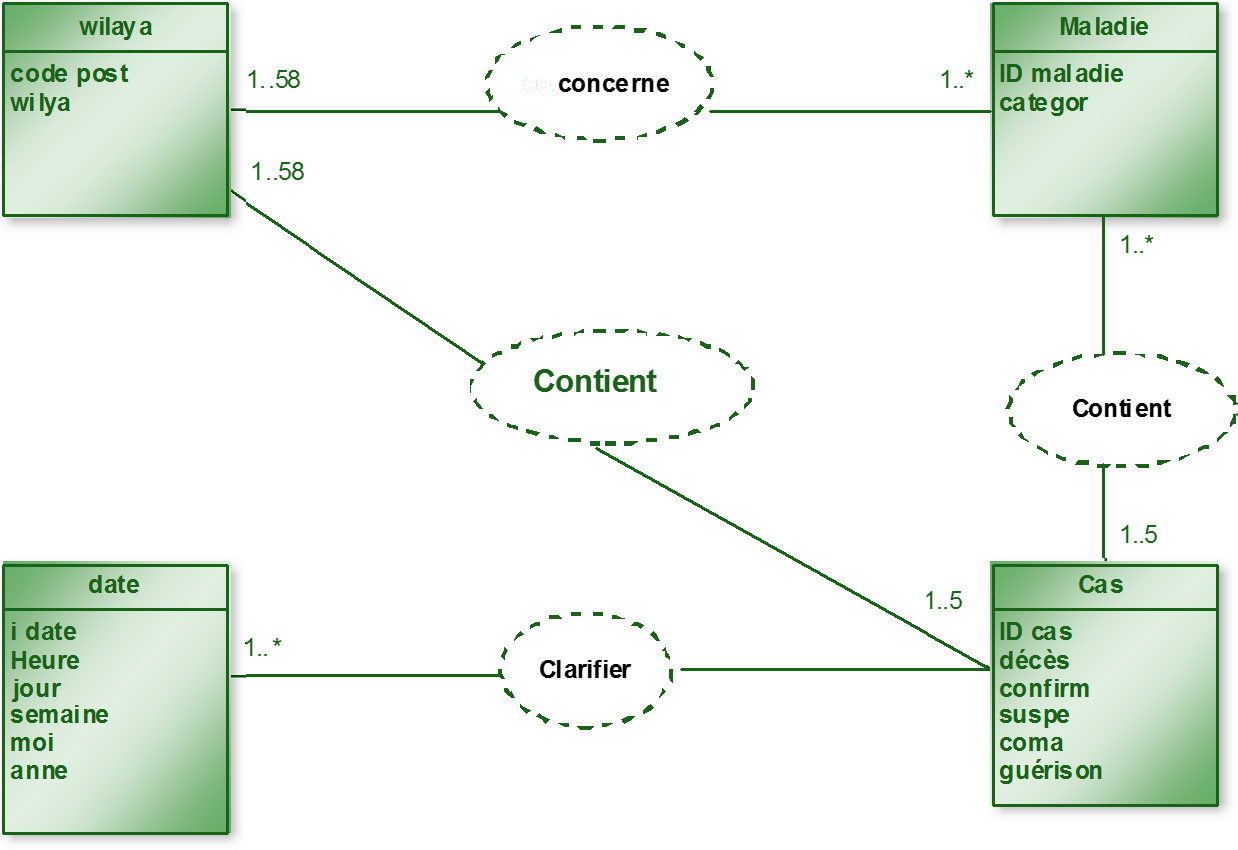
\includegraphics[width=\textwidth]{Chapitre3/entitymodel.png}}
        \caption{\label{fig:my-label} The association entity model}
     \end{figure}
     

\section{Choose a good web host}
Domain name is like the address and the CMS is like the materials you build your site with, but the web host is the actual parcel where your website exists online.\\
Some are free and come with bandwidth limitations or built-in ads, but there are also commercial options that work much better. Many hosts also provide server security features that can better protect your site data.\\
Our project is hosted in github Pages.


\section{Use a firewall}
As soon as your website is online, it is exposed to cyber threats. Automated bots search for vulnerable websites, and newly created sites are a particularly tempting target.\\

Adding a web application firewall (WAF), such as Cloudbric, Incapsula, or Cloudflare, will secure your website before attacks start.

\newpage
\section{Database schema:}
Above a schema of our Database 

\begin{figure}[!htb]
        \center{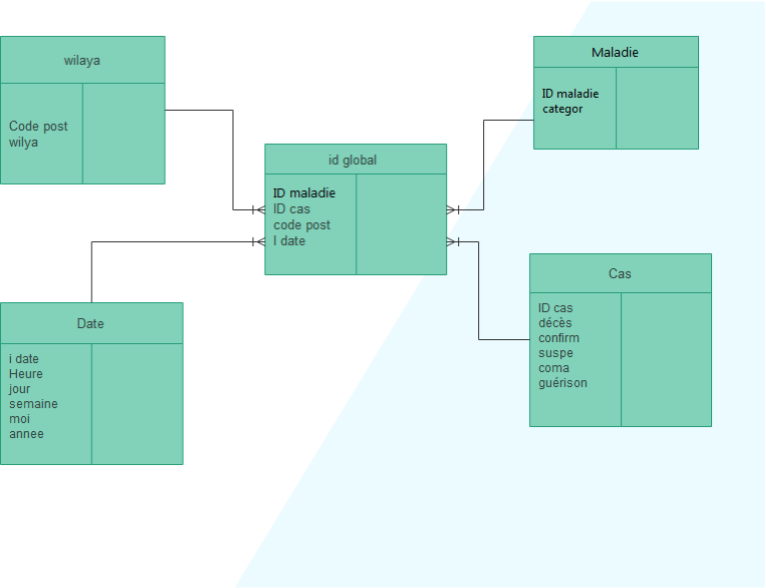
\includegraphics[width=\textwidth]{Chapitre3/db.png}}
        \caption{\label{fig:dbschema} Db Schema}
     \end{figure}
\newpage     
\section{HCI (IHM)}
According to the basic criteria of the ergonomics of the interfaces \cite{bastien1998ergonomie}, we build our Webapp as a dasshoard for a \textit{Guidance}, \textit{Explicity} with charts and Maps, \textit{Adaptability} 
\begin{figure}[!htb]
        \center{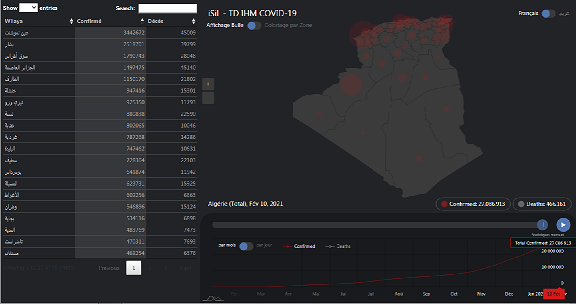
\includegraphics[width=\textwidth]{Chapitre3/dzdash.png}}
        \caption{\label{fig:dashboard} DashBoard}
     \end{figure}
